\documentclass[class=article, crop=false, 12pt]{standalone}
\usepackage[subpreambles=true]{standalone}
\usepackage{../.common/common}
\allowdisplaybreaks % equation environment from amsmath can break equation between page


\author{Tony Shing}
%\pretitle{Supplementary}

\topic{Note 6A (Mechanics)}
\title{Vectors in Polar Coordinates}

\version{2025} % leave blank for omitting

\begin{document}

\maketitle

%\heading{Lecture}{Tony}

\begin{overview}
    \begin{itemize}
        \item The unit vectors in polar coordinate are not "constant" of position and time.
        \item Angular quantities ($\theta/\omega/\alpha$) $\sim$ Angular component of ($s/v/a$). 
        \item Relative angular velocity does not exists because it is only the angular component.
    \end{itemize}
\end{overview}



% content begins here
% Section %%%%%%%%%%%%%%%%%%%%%%%%%%%%%%%%%%%%%%%%%%%%%%%%%%%%
\section{The Vector Expressions}

\subsection{Unit Vectors as function of coordinate}

In x-y coordinate, every vector can be expressed in terms of the two unit vectors $\{\hhat{x}, \hhat{y}\}$ and their components.
\aleq{
    \vvec{s} = s_x \hhat{x} + s_y \hhat{y}
}

When switching into polar coordinate, we wish to do the same, 
but with two different unit vectors $\{\hhat{r}, \hhat{\theta}\}$.
\aleq{
    \vvec{s} = s_r \hhat{r} + s_\theta \hhat{\theta}
}

The problem about $\{\hhat{r}, \hhat{\theta}\}$ is that their directions depends on the coordinate $(r, \theta)$. 
We require:
\begin{itemize}
    \item $\hhat{r}$ should always be radially outward, 
    i.e. extend from the origin to the current point.
    
    \item $\hhat{\theta}$ should always be perpendicular to $\hhat{r}$, 
    like an anti-clockwise torque. 
    
\end{itemize}

\begin{center}
    \begin{minipage}{0.3\linewidth}
        \centering
        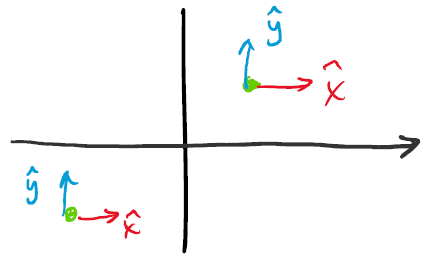
\includegraphics[width=\textwidth]{unit_xy}
    \end{minipage}
    \hspace{0.05\textwidth}
    v.s.
    \hspace{0.05\textwidth}
    \begin{minipage}{0.3\linewidth}
        \centering
        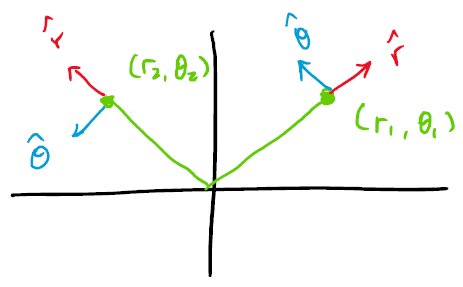
\includegraphics[width=\textwidth]{unit_rth}
    \end{minipage}
\end{center}


From the figure, we can see that the pairs of unit vectors at different positions are pointing in different directions. 
Notation-wise we should write them as:
\aleq{
    \hhat{r}_\green{\text{at }(r_1, \theta_1)} \neq \hhat{r}_\green{\text{at }(r_2, \theta_2)} 
    \quad, \quad
    \hhat{\theta}_\green{\text{at }(r_1, \theta_1)} \neq \hhat{\theta}_\green{\text{at }(r_2, \theta_2)} 
}

\begin{center}
    \begin{minipage}{0.55\textwidth}
        \begin{framed}
            \centering
            The unit vectors are functions of coordinates. 
        \end{framed}
    \end{minipage}
\end{center}

Unfortunately, this "\green{at $(r,\theta)$}" is almost NEVER emphasized in regular textbooks.

\newpage
This makes a big difference in vector differentiation.
We can show this by product rules: 
\begin{itemize}
    \item \bf{\ul{Vector in terms of $\{\hhat{x}, \hhat{y}\}$}}\\
    \cul[red]{$\hhat{x},\hhat{y}$ always point in the same direction,
    independent of position. }
    They can be treated as constants. $\Rightarrow$ Differentiation = 0.
    \aleq{
        \vvec{s} &= s_x \hhat{x} + s_y \hhat{y} \\[1ex]
        \dv{\vvec{s}}{t} 
        &= \dv{s_x}{t}\hhat{x} + s_x\tkn{xh}{\red{\ul{\dv{\hhat{x}}{t}}}} 
            + \dv{s_y}{t}\hhat{y} + s_y\tkn{yh}{\red{\ul{\dv{\hhat{y}}{t}}}}
    }
    \addArrow[red]{xh}{(0,-2ex)}{$\scriptstyle =0$}{(0, -2.5ex)}
    \addArrow[red]{yh}{(0,-2ex)}{$\scriptstyle =0$}{(0, -2.5ex)} 
    

    \item \bf{\ul{Vector in terms of $\{\hhat{r}, \hhat{\theta}\}$}}\\
    \cul[blue]{$\hhat{r}, \hhat{\theta}$ shall be functions of position $(r, \theta)$.}
    Then along a trajectory, $(r, \theta)$ are functions of $t$.
    $\Rightarrow$ Differentiating them against $t$ can be non-zero.
    \aleq{
        \vvec{s} &= s_r\hhat{r} + s_\theta\hhat{\theta} \\[1ex]
        \dv{\vvec{s}}{t} &= \dv{s_r}{t}\hhat{r} + s_r \tkn{rh}{\blue{\ul{\dv{\hhat{r}}{t}}}}
                            + \dv{s_\theta}{t}\hhat{\theta} + s_\theta \tkn{th}{\blue{\ul{\dv{\hhat{\theta}}{t}}}}
    }
    \addArrow[blue]{rh}{(0,-2ex)}{$\substack{\hhat{r}\text{ is a function of } \\ r\text{ \& }\theta}$}{(0, -2.5ex)}{(0,-1ex)}
    \addArrow[blue]{th}{(0,-2ex)}{$\substack{\hhat{\theta}\text{ is a function of } \\ r\text{ \& }\theta}$}{(0, -2.5ex)}{(0,-1ex)}

\end{itemize}

\vskip 1.5em
\bf{\ul{Note 1}}: The above are just product rules, but applied on (component)$\times$(unit vector).\\

\bf{\ul{Note 2}}: In general, unit vectors are functions of coordinate for any non-rectangular coordinate.

\begin{center}
    E.g. 
    \begin{minipage}{0.4\linewidth}
        \centering
        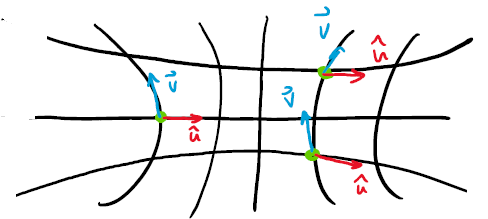
\includegraphics[width=\textwidth]{unit_curve}
    \end{minipage}
    \\[1ex]
    \it{(This is also the thing which physicists need to solve in general relativity.)}
\end{center}



%%%%%%%%%%%%%%%%%%%
\subsection{Differentiation on Polar Unit Vectors}

Because $\{\hhat{x}, \hhat{y}\}$ never change by position, 
we usually call a rectangular coordinate as \bf{"ambient coordinate"},
and use them as a reference to express other unit vectors. 
To tell how to differentiate the polar unit vectors, 
we can \cul[red]{first express them in the $\bigcirc\hhat{x} + \square\hhat{y}$ form, 
then differentiation} \cul[red]{is solely on the components.}

\begin{enumerate}
    \item We can relate $\{\hhat{r}, \hhat{\theta}\}$ and $\{\hhat{x}, \hhat{y}\}$ by trigonometry:
    \begin{center}
        \begin{minipage}{0.4\linewidth}
            \aleq{
                \Acboxed{
                    \begin{cases}
                        \hhat{r}_\green{\text{at }(r,\theta)} = (\cos\theta)\hhat{x} + (\sin\theta)\hhat{y} \\[1ex]
                        \hhat{\theta}_\green{\text{at }(r,\theta)} = (-\sin\theta)\hhat{x} + (\cos\theta)\hhat{y}
                    \end{cases}
                }
            }
        \end{minipage}
        \hspace{0.05\textwidth}
        \begin{minipage}{0.3\linewidth}
            \centering
            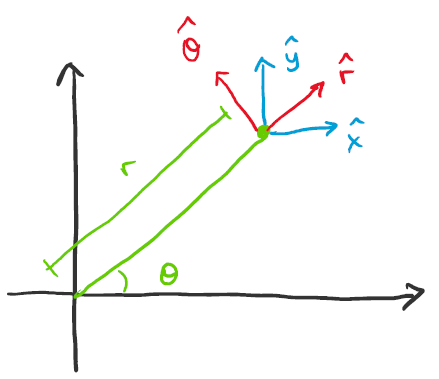
\includegraphics[width=\textwidth]{xy_rth}
        \end{minipage}
    \end{center}

    \begin{proof}
        It can be proven by just drawing triangles and play with sine/cosine. 
        But here I would like to provide you a method using vector properties.

        \begin{itemize}
            \item $\hhat{r}$ is a radial unit vector and its projection to $\hhat{x}$ and $\hhat{y}$ are just cosine and sine.
            \aleq{
                \hhat{r}\cdot \hhat{x} = \norm{\hhat{r}}\cos\theta = \cos\theta
                \qquad &\text{and}\qquad 
                \hhat{r}\cdot \hhat{y} = \norm{\hhat{r}}\sin\theta = \sin\theta \\
                %
                &\ \Downarrow \\
                %
                \hhat{r}_\green{\text{at }(r,\theta)} 
                    = (\hhat{r}\cdot\hhat{x})\hhat{x} + (\hhat{r}\cdot\hhat{y})\hhat{y} &\,= (\cos\theta)\hhat{x} + (\sin\theta)\hhat{y}
            }

            \item We want $\hhat{\theta}$ to be perpendicular to $\hhat{r}$ and also have a length of $1$.
            Let $\hhat{\theta} = (\theta_x) \hhat{x} + (\theta_y) \hhat{y}$, then
            \aleq{
                \hhat{\theta}\cdot\hhat{r} = (\theta_x)(\cos\theta) + (\theta_y)(\sin\theta) &= 0
                \qquad \text{and}\qquad 
                (\theta_x)^2 + (\theta_y)^2 = 1 \\
                %
                &\ \Downarrow \\
                %
                \theta_x= -\sin\theta
                \qquad &\text{and}\qquad 
                \theta_y = \cos\theta \\
                %
                &\ \Downarrow \\
                %
                \hhat{\theta}_\green{\text{at }(r,\theta)} = (-\sin&\theta)\hhat{x} + (\cos\theta)\hhat{y}
            }
        \end{itemize}
        
    \end{proof}

    \item From the relation, we can see that $\hhat{r}$ and $\hhat{\theta}$ are function to $\theta$ only. So
    \aleq{
        \Aboxed{
            \green{\eval{\black{\pdvv{\hhat{r}}{r}}}_{\text{at }(r,\theta)}} 
            = \green{\eval{\black{\pdvv{\hhat{\theta}}{r}}}_{\text{at }(r,\theta)}} 
            = 0
        }
    }

    and differentiating on $\theta$ gives
    \aleq{
        \Aboxed{
        \begin{cases}
            \green{\eval{\black{\pdvv{\hhat{r}}{\theta}}}_{\text{at }(r,\theta)}} 
                = -\sin\theta \hhat{x} + \cos\theta \hhat{y} = \hhat{\theta}_\green{\text{at }(r,\theta)} \\[1.2em]
            %
            \green{\eval{\black{\pdvv{\hhat{\theta}}{\theta}}}_{\text{at }(r,\theta)}} 
                = -\cos\theta \hhat{x} - \sin\theta \hhat{y} = -\hhat{r}_\green{\text{at }(r,\theta)}
        \end{cases}
        }
    }
    \cul[red]{Differentiating the two unit vectors by $\theta$ results in each other!}
    This numerical coincident is related to rotational symmetry.

    \item If the positions $(r,\theta) = (r(t),\theta(t))$ are functions of time $t$,
    the differentiation with respect to $t$ can be computed by the (partial-D) chain rule:
    \aleq{
        \Aboxed{
        \begin{cases}
            \green{\eval{\black{\pdvv{\hhat{r}}{t}}}_{\text{at }(r,\theta)}} 
                = \cancel{\pdvv{\hhat{r}}{r}}\dvv{r}{t} + \pdvv{\hhat{r}}{\theta}\dvv{\theta}{t} 
                = \dvv{\theta}{t}\cdot\hhat{\theta}_\green{\text{at }(r,\theta)} \\[1em]
            %
            \green{\eval{\black{\pdvv{\hhat{\theta}}{t}}}_{\text{at }(r,\theta)}} 
                = \cancel{\pdvv{\hhat{\theta}}{r}}\dvv{r}{t} + \pdvv{\hhat{\theta}}{\theta}\dvv{\theta}{t} 
                = -\dvv{\theta}{t}\cdot\hhat{r}_\green{\text{at }(r,\theta)}
        \end{cases}
        }
    }

\end{enumerate}





\linesep
% Section %%%%%%%%%%%%%%%%%%%%%%%%%%%%%%%%%%%%%%%%%%%%%%%%%%%%
\section{Kinematic Quantities in terms of $(r,\theta)$}

\subsection{Position Vector}


A position vector in the $\bigcirc\hhat{x} + \square\hhat{y}$ form has its components equal to the coordinate it is pointing to, i.e.
\aleq{
    \text{Pointing at coordinate }(X,Y) \quad\Leftrightarrow\quad \text{ Expression }=X\hhat{x} + Y\hhat{y} 
}

But \cul[red]{this is not true for vector expressed in other coordinates}. E.g. 
\aleq{
    \text{Pointing at polar coordinate }(R,\Theta) \quad\cxcancel[red]{\Leftrightarrow}\quad \text{ Expression }=R\hhat{r}+\Theta\hhat{\theta} 
}

For proper conversion, we must first use the conversion between the unit vectors. 
Observed their relations can be written as a matrix:
\aleq{
    \bmat{\hhat{r} \\ \hhat{\theta}}
    =
    \bmat{\cos\theta & \sin\theta \\ -\sin\theta & \cos\theta}
    \bmat{\hhat{x} \\ \hhat{y}}
}

This square matrix $\bmat{\cos\theta & \sin\theta \\ -\sin\theta & \cos\theta}$ is known as the "\bf{rotation matrix}", 
which when multiplied to a vector, 
will geometrically rotate the vector about the origin by an angle $\theta$. 
Its inverse is trivial - 
by replacing $\theta$ to $-\theta$. 
(reverse of clockwise rotation = anticlockwise rotation)
One can easily check that:
\aleq{
    \bmat{\cos\theta & -\sin\theta \\ \sin\theta & \cos\theta}
    \bmat{\cos\theta & \sin\theta \\ -\sin\theta & \cos\theta}
    =\bmat{1 & 0 \\ 0 & 1}
}

\begin{center}
    \begin{minipage}{0.7\linewidth}
        \centering
        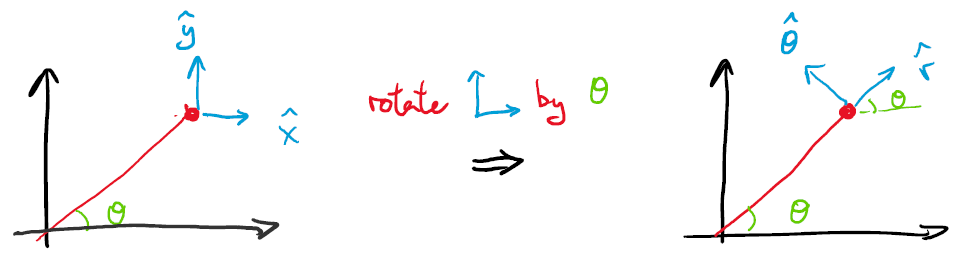
\includegraphics[width=\textwidth]{rotate_xy}
    \end{minipage}
\end{center}

Substitute this into a position vector tells us how to write a position vector properly
 by its polar coordinate $(r, \theta)$ and unit vectors $\{\hhat{r}, \hhat{\theta}\}$.
\aleq{
    \vvec{r} &= x\hhat{x} + y\hhat{y} \\
    &= \bmat{x & y} \bmat{\hhat{x} \\ \hhat{y} }\\
    &= \bmat{x & y} 
        \bmat{\cos\theta & -\sin\theta \\ \sin\theta & \cos\theta}
        \bmat{\cos\theta & \sin\theta \\ -\sin\theta & \cos\theta}
        \bmat{\hhat{x} \\ \hhat{y}}\\
    &= \bmat{x & y}\bmat{\cos\theta & \sin\theta \\ \sin\theta & \cos\theta}
        \bmat{\hhat{r} \\ \hhat{\theta}}\\
    &= \bmat{x\cos\theta+y\sin\theta & -x\sin\theta + y\cos\theta}
        \bmat{\hhat{r} \\ \hhat{\theta}}\\
    &= \bmat{(r\cos\theta)\cos\theta + (r\sin\theta)\sin\theta & -(r\cos\theta)\sin\theta + (r\sin\theta)\cos\theta}
        \bmat{\hhat{r} \\ \hhat{\theta}}\\
    &= \bmat{r & 0 } \bmat{\hhat{r} \\ \hhat{\theta}}\\
    \Aboxed{\vvec{r} &= r\hhat{r}}
}

So the proper way to write a vector in terms of its polar coordinate is 
... \bf{just by its radial component.} Isn't that weird?\\

Normally when we describe a point on a 2D plane, 
we need two information - its $x$ and $y$ components.
Why is there only 1 information ($r$ component) in the polar form? 
This is because the second piece of information is hidden in the unit vector $\hhat{r}$:
\aleq{
    \vvec{r} = r \tkn{rhat}{\cul[yellow]{\hhat{r}}}
    \qquad\qquad\xRightarrow{\text{writing more accurately}}\qquad 
    \vvec{r} = r\cdot \hhat{r}_{\green{\text{at }(r,\tkn{rhat2}{\ul{\theta}})}}
}
\addArrow[yellow]{rhat}{(0,-2.5ex)}{which direction?}{(0,-0.5ex)}{(0,-0.5ex)}
\addArrow[green]{rhat2}{(0,-2.5ex)}{in $\theta$ direction!}{(0,-0.5ex)}{(0,-0.5ex)}

\vskip 1em
We cannot really tell which direction $\hhat{r}$ is pointing to, 
if we do not know the "$\green{\text{at }(r,\theta)}$" part.\\

As a comparison in x-y coordinate, 
we almost never care about the two unit vectors because we always know that 
$\hhat{x}$ is the one pointing horizontally and $\hhat{y}$ is the one pointing vertically.
\aleq{
    \vvec{r} = x\cdot \tkn{xhat}{\cul[red]{\hhat{x}}} + y\cdot \tkn{yhat}{\cul[blue]{\hhat{y}}}
}
\addArrow[red]{xhat}{(-3ex,-2.5ex)}{always\\horiztonal}{(0,-1ex)}{(0,-1.5ex)}
\addArrow[blue]{yhat}{(3ex,-2.5ex)}{always\\vertical}{(0,-1ex)}{(0,-1.5ex)}

\vskip 2em
\begin{notation}
    2D coordinates are represented by $(x,y)$ and $(r,\theta)$. Their conversion is according to the position vector's component: 
        \aleq{
            \vvec{r} = x\hhat{x}+y\hhat{y} = (r\cos{\theta})\hhat{x}+(r\sin{\theta})\hhat{y} = r\hhat{r}
        }
        Note that 
        \begin{itemize}
            \item $\vvec{r}$ = {\bf{position vector}}
            \item $r$ = {\bf{radial component}}
            \item $\hhat{r}$ = {\bf{radial unit vector}}
        \end{itemize} 
        In polar coordinate, \red{\bf{length of position vector $\norm{\vvec{r}} = r$}} exactly.

\end{notation}


%%%%%%%%%%%%%%%%%%%%%%%%%%%%%%%%%%%%%%%
\subsection{Displacement Vector}

Displacement vector is the subtraction between two position vector. 
In x-y coordinate, the subtraction is simply done within the components:
\aleq{
    \vvec{r}_2 - \vvec{r}_1 = (x_2 \hhat{x} + y_2\hhat{y}) - (x_1\hhat{x} + y_1\hhat{y}) = [x_2 - x_1]\hhat{x} + [y_2 - y_1]\hhat{y} 
}

But in polar form, you cannot!
\aleq{
    \vvec{r}_2 - \vvec{r}_1 = (r_2\hhat{r}) - (r_1\hhat{r}) \neq [r_2-r_1]\hhat{r}
}

This is the fault of omitting the "$\green{\text{at }(r,\theta)}$" part. 
Remember, $\hhat{r}$ at different position are differnt vectors. 
The true component subtraction will require a lot of trigonometry. 

\begin{center}
    \begin{minipage}{0.4\linewidth}
        \centering
        \aleq{
            \vvec{r}_2 - \vvec{r}_1 = 
            (r_2\cdot \hhat{r}_\green{\text{at }(r_2,\theta_2)}) - (r_1 \cdot \hhat{r}_\green{\text{at }(r_1,\theta_1)}) 
            = (\text{Awful!})
        }
    \end{minipage}
    \hspace{0.05\textwidth}
    \begin{minipage}{0.3\linewidth}
        \centering
        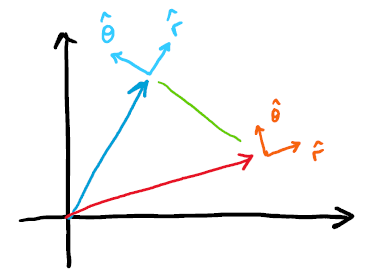
\includegraphics[width=\textwidth]{nasty_trigo}
    \end{minipage}
\end{center}


Furthermore, if we really try to subtract by component, 
the result "vector" on the polar grid is not even a straightline. 
(This happens in every curved coordinate system.)
\begin{center}
    \begin{minipage}{0.25\linewidth}
        \centering
        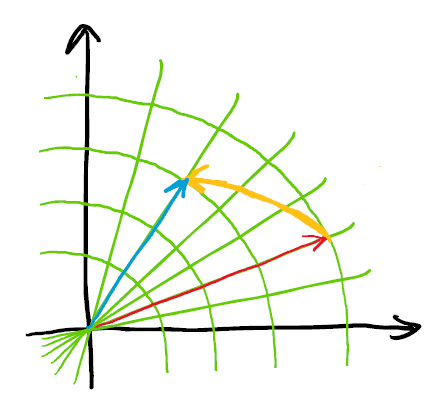
\includegraphics[width=\textwidth]{not_straight_1}
    \end{minipage}
    \begin{minipage}{0.4\linewidth}
        \centering
        \yellow{Not a straight line.\\
        Cannot even call it a vector.}
    \end{minipage}
    \begin{minipage}{0.2\linewidth}
        \centering
        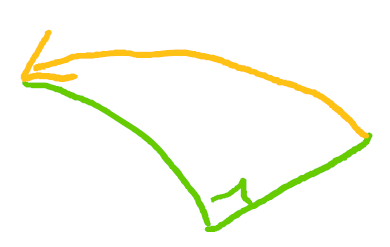
\includegraphics[width=0.9\textwidth]{not_straight_3}
    \end{minipage}
\end{center}

The only valid definition is the \bf{infinitestimal displacement vector}, 
i.e. when we subtract two very close vector, 
their difference is approximately a straight line and we can take limit to its length to $0$. 
\begin{center}
    \begin{minipage}{0.4\linewidth}
        \centering
        \aleq{
            \dd{\vvec{r}} &= \dd{\qty(r\hhat{r}_\green{\text{at }(r,\theta)})} \\
            &= \dd{(r)}\cdot \hhat{r}_\green{\text{at }(r,\theta)} + r\cdot \dd\qty(\hhat{r}_\green{\text{at }(r,\theta)})\\
            \Aboxed{
                \dd{\vvec{r}} &= \dd{(r)}\cdot \hhat{r}_\green{\text{at }(r,\theta)} 
                    + r\cdot \dd{(\theta)} \cdot \hhat{\theta}_\green{\text{at }(r,\theta)}
            }
        }
    \end{minipage}
    \hspace{0.05\textwidth}
    \begin{minipage}{0.3\linewidth}
        \centering
        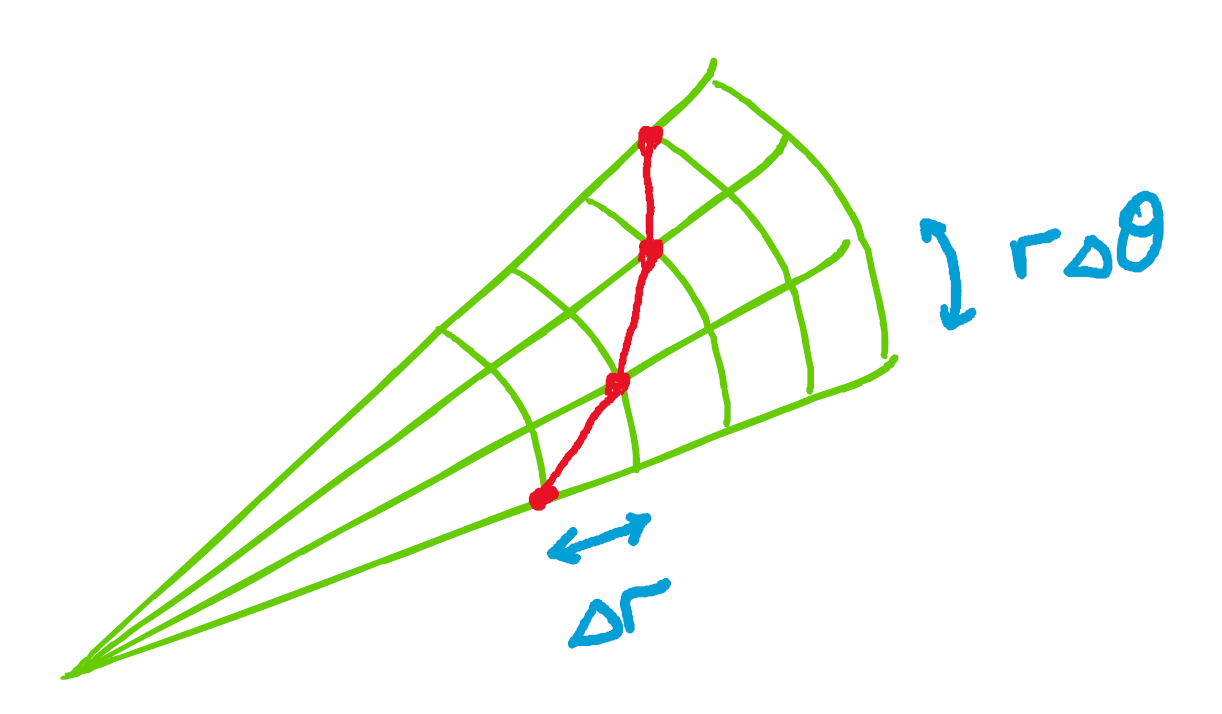
\includegraphics[width=\textwidth]{not_straight_2}
    \end{minipage}
\end{center}


The differential $\dd{(\hhat{r}_\green{\text{at }(r,\theta)})}$ comes from 
$\dvv{\hhat{r}}{\theta} = \hhat{\theta}$ which is derived previously. 
In textbooks you will usually find the form without "$\green{\text{at }(r,\theta)}$", 
which is
\aleq{
    \Aboxed{
        \dd{\vvec{r}} = (\dd{r})\hhat{r} + (r\dd{\theta})\hhat{\theta}
    }
}




%%%%%%%%%%%%%%%%%%%%%%%%%%%%%%%%%%
\subsection{Velocity Vector}

Velocity is defined by displacement divided by period of time $\Delta t$, and then taking $\Delta t \to 0$.
From the infinitestimal displacement, we immediately get
\aleq{
    \vvec{v} &= \lim_{\Delta t \to 0} \frac{\vvec{r}(t)}{\Delta t} \\[1em]
    &= \dv{\vvec{r}(t)}{t} \\
    \Aboxed{
        \vvec{v} &= \dv{r}{t}\cdot \hhat{r}_\green{\text{at }(r,\theta)} 
            + r\cdot \dv{\theta}{t} \cdot \hhat{\theta}_\green{\text{at }(r,\theta)}
    }
}

We can identify the two components of a velocity vector. 
It is common to denote $\dvv{\theta}{t} = \omega$ as the angular speed.


\begin{minipage}{0.5\linewidth}
    \aleq{
        \vvec{v} &= v_r \hhat{r} + v_\theta \hhat{\theta} \\[1ex]
        &= \qty(\dv{r}{t}) \hhat{r} + \qty(r\dv{\theta}{t}) \hhat{\theta} \\[1ex]
        &= v_r\hhat{r} + r\omega \hhat{\theta} 
    }
\end{minipage}
\hspace{0.05\textwidth}
\begin{minipage}{0.2\linewidth}
    \centering
    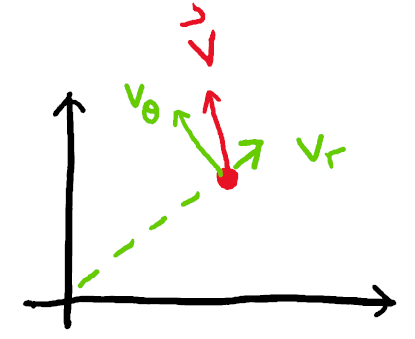
\includegraphics[width=\textwidth]{v_component}
\end{minipage}




\vskip 3.5em
%%%%%%%%%%%%%%%%%%%%%%%%%%%%%%%%%%
\subsection{Acceleration Vector}

Acceleration is defined by differentiating the velocity once again. 
But with $\hhat{r}$ and $\hhat{\theta}$ being function of $t$ as well, 
the full expansion gives a lengthy product rule.
\aleq{
    \vvec{a}(t) &= \dv{\vvec{v}(t)}{t} \\[1em]
    %
    &= \dv{t}\qty(\dv{r}{t}\cdot \hhat{r}_\green{\text{at }(r,\theta)} 
    + r\cdot \dv{\theta}{t} \cdot \hhat{\theta}_\green{\text{at }(r,\theta)}) \\[1.2em]
    %
    &= \dv[2]{r}{t}\cdot\hhat{r}_\green{\text{at }(r,\theta)} 
        + \dv{r}{t}\cdot \cus[red]{\dv{t}\qty(\hhat{r}_\green{\text{at }(r,\theta)})}{\dv{\hhat{r}}{t}=\dv{\theta}{t}\hhat{\theta}}
        + \dv{r}{t}\cdot\dv{\theta}{t} \cdot \hhat{\theta}_\green{\text{at }(r,\theta)} 
        + r\cdot \dv[2]{\theta}{t}\cdot \hhat{\theta}_\green{\text{at }(r,\theta)} 
        + r\cdot \dv{\theta}{t} \cdot \cus[red]{\dv{t}\qty(\hhat{\theta}_\green{\text{at }(r,\theta)})}{\dv{\hhat{\theta}}{t}=-\dv{\theta}{t}\hhat{r}} \\[1.2em]
    %
    &= \dv[2]{r}{t}\cdot\hhat{r}_\green{\text{at }(r,\theta)} 
        + \dv{r}{t}\cdot\cul[red]{\dv{\theta}{t}\cdot\hhat{\theta}_\green{\text{at }(r,\theta)}}
        + \dv{r}{t}\cdot\dv{\theta}{t} \cdot \hhat{\theta}_\green{\text{at }(r,\theta)} 
        + r\cdot \dv[2]{\theta}{t}\cdot \hhat{\theta}_\green{\text{at }(r,\theta)} 
        \cul[red]{-} r\cdot \dv{\theta}{t} \cdot \cul[red]{\dv{\theta}{t}\cdot \hhat{r}_\green{\text{at }(r,\theta)}} \\[1.2em]
    %
    &= \qty[\dv[2]{r}{t} - r\cdot \qty(\dv{\theta}{t})^2]\hhat{r}_\green{\text{at }(r,\theta)}
    + \qty[2\dv{r}{t}\cdot\dv{\theta}{t} + r\cdot \dv[2]{\theta}{t}]\hhat{\theta}_\green{\text{at }(r,\theta)}
} 

\newpage
There are 4 terms in total. Notation-wise we identify them as:
\begin{enumerate}
    \item \it{(Along $\hhat{r}$)} \bf{\ul{Radial acceleration}} : $\displaystyle \dv[2]{r}{t}$
    
    \item \it{(Along $\hhat{r}$)} \bf{\ul{Centripetal acceleration}} : $\displaystyle - r\cdot \qty(\dvv{\theta}{t})^2 = -r\cdot \omega^2$\\
    \blue{Minus sign for pointing toward origin.}
    
    \item \it{(Along $\hhat{\theta}$)} \bf{\ul{Coriolis acceleration}} : $\displaystyle 2\dv{r}{t}\cdot\dvv{\theta}{t} = 2 v_r\cdot \omega$\\
    \blue{This term appears only if radial distance is changing, i.e. $\dv{r}{t}\neq 0$.}
    
    \item \it{(Along $\hhat{\theta}$)} \bf{\ul{Euler acceleration}} : $\displaystyle r\cdot \dv[2]{\theta}{t} = r\alpha$\\
    \blue{This term appears only if the angular speed is accelerating, i.e. $\dv[2]{\theta}{t} \neq 0$.}
\end{enumerate}

They are also the \red{\bf{4 pseudo-acceleration}} terms in a rotating reference frame.


\vskip 2em
%%%%%%%%%%%%%%%%%%%%%%%%%%%%%%%%%%
\subsection{The Angular Quantities}

Observe that if we perform cross product to a vector with its position vector, 
we essentially \ul{remove its radial component} and only leave the angular compoenet. Because
\aleq{
    \bcase{
        \hhat{r}_\green{\text{at }(r,\theta)} \cross \hhat{r}_\green{\text{at }(r,\theta)} &= \cul[red]{0} \tkm{cross0}\\
        \hhat{r}_\green{\text{at }(r,\theta)} \cross \hhat{\theta}_\green{\text{at }(r,\theta)} & = \hhat{z}\tkm{zhat}
    }
}
\addArrow[red]{cross0}{(6ex,0)}{\scriptsize Cross product with itself = 0}{(1ex,0.5ex)}{(10ex,0)}
\addArrow{zhat}{(8ex,0)}{\scriptsize $\hhat{z}$ is independent\\[-1ex]\scriptsize of position}{(1ex,0.5ex)}{(4ex,0)}


So for a general vector $\vvec{s}$,
\aleq{
    \hhat{r}_\green{\text{at }(r,\theta)} \cross \vvec{s} 
    &= \hhat{r}_\green{\text{at }(r,\theta)} \cross (s_r \hhat{r}_\green{\text{at }(r,\theta)} 
        + s_\theta \hhat{\theta}_\green{\text{at }(r,\theta)}) \\
    &= s_r(\hhat{r}_\green{\text{at }(r,\theta)} \cross \hhat{r}_\green{\text{at }(r,\theta)}) 
        + s_\theta(\hhat{r}_\green{\text{at }(r,\theta)} \cross \hhat{\theta}_\green{\text{at }(r,\theta)})\\
    &= 0 + \tkn{thcomponent}{\cul[red]{s_\theta}} \hhat{z}
}
\addArrow[red]{thcomponent}{(0,-2ex)}{\scriptsize Successfully filter out\\[-1ex]\scriptsize the $\theta$ component}
{(0,-1ex)}{(0,-1.5ex)}

\hfill\\[1em]
Apply this on our displacement / velocity / acceleration vector will give the familiar definitions of 
angular displacement / angular velocity / angular acceleration.

\begin{enumerate}
    \item \bf{\ul{Angular position vector:}}\\[1ex]
    Such thing does not exist, 
    because position vector does not have angular component. 
    \aleq{
        \hhat{r}_\green{\text{at }(r,\theta)}\cross\vvec{r} 
        = r(\hhat{r}_\green{\text{at }(r,\theta)}\cross\hhat{r}_\green{\text{at }(r,\theta)})=0
    }
    
    \item \bf{\ul{Angular displacement vector:}}\\[1ex]
    Only exists in the infinitestimal version.
    \aleq{
        \hhat{r}_\green{\text{at }(r,\theta)}\cross\dd{\vvec{r}} 
        = (\dd{r})\cancelto{0}{\hhat{r}_\green{\text{at }(r,\theta)}\cross\hhat{r}_\green{\text{at }(r,\theta)}} 
            + (r\dd{\theta})\hhat{r}_\green{\text{at }(r,\theta)}\cross\hhat{\theta}_\green{\text{at }(r,\theta)}
        = r\dd{\theta}\hhat{z}
    }

    The infinitestimal angular displacement vector is formally defined in $\hhat{z}$ direction:
    \aleq{
        \Acboxed{
            \dd{\vvec{\theta}} = (\dd{\theta})\hhat{z} 
            = \frac{\hhat{r}_\green{\text{at }(r,\theta)}\cross\dd{\vvec{r}}}{r} 
            = \frac{(\text{Angular component of }\dd{\vvec{r}})}{r}\hhat{z}
        }
    }
    
    \begin{minipage}{0.55\linewidth}
        Its magnitude yields $\displaystyle \dd{\theta} = \frac{\norm{\dd{\vvec{r}}}}{r} = \frac{\text{arc length}}{\text{radius}}$.
    \end{minipage}
    \hspace{0.01\textwidth}
    \begin{minipage}{0.42\linewidth}
        \centering
        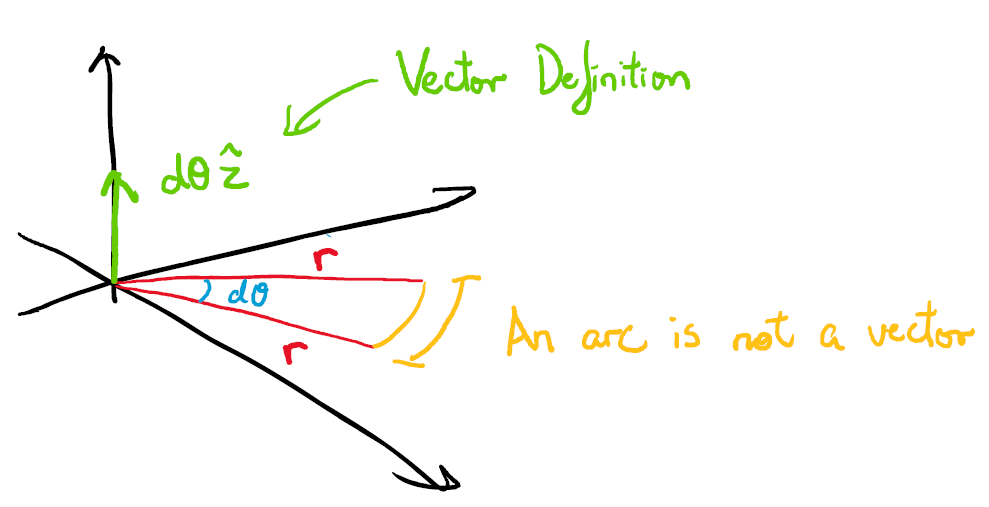
\includegraphics[width=\textwidth]{angular_theta}
    \end{minipage}

    \item \bf{\ul{Angular velocity vector:}}
    \aleq{
        \hhat{r}_\green{\text{at }(r,\theta)}\cross\vvec{v} &= \dv{r}{t}\cdot \cancelto{0}{\hhat{r}_\green{\text{at }(r,\theta)}\cross\hhat{r}_\green{\text{at }(r,\theta)}} 
        + r\cdot \dv{\theta}{t} \hhat{r}_\green{\text{at }(r,\theta)}\cross \hhat{\theta}_\green{\text{at }(r,\theta)}\\[0.5em]
        &= r\dv{\theta}{t}\hhat{z}
    }
    The angular velocity vector is formally defined in $\hhat{z}$ direction:
    \aleq{
        \Acboxed{
            \vvec{\omega} = \omega \hhat{z} = \dv{\theta}{t}\hhat{z} 
            = \frac{\hhat{r}_\green{\text{at }(r,\theta)}\cross\vvec{v}}{r} =\frac{(\text{Angular component of }\vvec{v})}{r}\hhat{z}
        }
    }
    

    \begin{minipage}{0.6\linewidth}
        Its magnitude yields our familiar definition $\displaystyle \omega = \frac{\norm{\vvec{v}}}{r}$.
    \end{minipage}
    \hspace{0.01\textwidth}
    \begin{minipage}{0.32\linewidth}
        \centering
        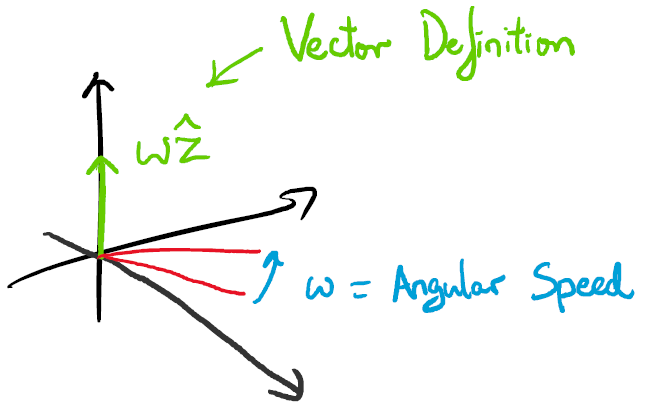
\includegraphics[width=\textwidth]{angular_v}
    \end{minipage}

    
    \item \bf{\ul{Angular acceleration vector:}}
    \aleq{
        \hhat{r}_\green{\text{at }(r,\theta)}\cross\vvec{a} &= 
        \qty[\dv[2]{r}{t} - r\cdot \qty(\dv{\theta}{t})^2]\cancelto{0}{\hhat{r}_\green{\text{at }(r,\theta)}\cross\hhat{r}_\green{\text{at }(r,\theta)}}
        + \qty[2\dv{r}{t}\cdot\dv{\theta}{t} + r\cdot \dv[2]{\theta}{t}]\hhat{r}_\green{\text{at }(r,\theta)}\cross\hhat{\theta}_\green{\text{at }(r,\theta)}\\[0.5em]
        &= \qty[2\dv{r}{t}\cdot\dv{\theta}{t} + r\cdot \dv[2]{\theta}{t}]\hhat{z}
    }
    Different from the above, the angular acceleration is defined as the \nth{2} derivative to the angular displacement and ignore the Coriolis term. 
    Therefore its definition is uglier. But most of its use cases are in pure rotation, which then the Coriolis term is $0$.
    \aleq{
        \Acboxed{
            \vvec{\alpha} = \alpha\hhat{z} = \dvv[2]{\theta}{t}\hhat{z} = \inv{r}\qty(\hhat{r}_\green{\text{at }(r,\theta)}\cross\vvec{a} - 2\dv{r}{t}\cdot\dv{\theta}{t}\hhat{z})
        }
    }
    %Its magnitude is $\displaystyle \alpha = \inv{r}\qty(\norm{\vvec{a}} - 2v_r\cdot\omega)$. 
    %When the radial distance is fixed, the Coriolis term vanishes and it recovers a prettier form $\displaystyle \alpha = \frac{\norm{\vvec{a}}}{r}$.
\end{enumerate}



%%%%%%%%%%%%%%%%%%%%%%%%%%%%%
\linesep
\section{Relative Rotation?}

A naïve example to talk about relative motion:
\begin{itemize}
    \item B sees an object A in the same car, moving at velocity $\vvec{V}_{AB}$. 
    \item C sees B in a car, moving at velocity $\vvec{V}_{BC}$.
    \item Then C sees object A moving at velocity $\vvec{V}_{AC}=\vvec{V}_{AB}+\vvec{V}_{BC}$. 
\end{itemize}


\begin{center}
    \begin{minipage}{0.3\linewidth}
        \centering
        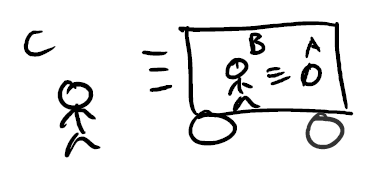
\includegraphics[width=\textwidth]{car}
    \end{minipage}
\end{center}

The above works in form of vector, 
i.e. it does not matter what trajectories are ABC actually moving in.
We can break it down component-wise if we write the velocities in x/y coordinate.
\aleq{
    \vvec{V}_{AC} &= \vvec{V}_{AB} + \vvec{V}_{BC}\\
    \qty(V_{AC,x}\hhat{x} + V_{AC,y}\hhat{y})
    &= \qty(V_{AB,x}\hhat{x} + V_{AB,y}\hhat{y}) 
        + \qty(V_{BC,x}\hhat{x} + V_{BC,y}\hhat{y})\\
    &= \qty(V_{AB,x}+V_{BC,x})\hhat{x} + \qty(V_{AB,y}+V_{BC,y})\hhat{y}
}

But in polar coordinate, \ul{angular velocity is only the angular component in the velocity vector}.
It does not make any sense if we add vectors just by one of their components.

\begin{center}
    \begin{minipage}{0.5\linewidth}
        \centering
        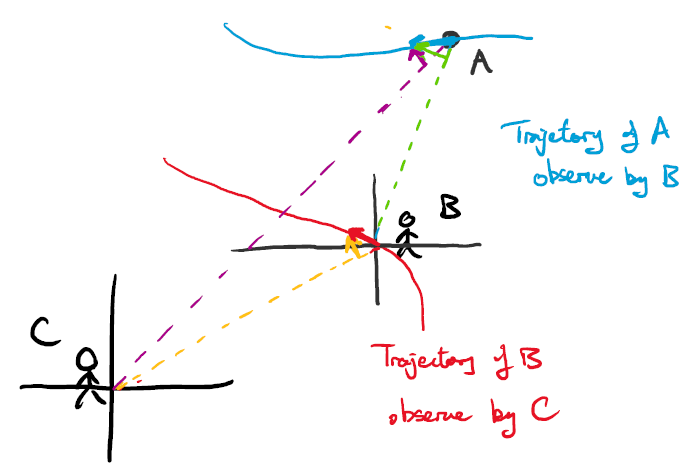
\includegraphics[width=\textwidth]{rel_traj}
    \end{minipage}
\end{center}


One must write 
\aleq{
    \vvec{V}_{AC} &= \vvec{V}_{AB} + \vvec{V}_{BC}\\
    \qty(V_{AC,r}\hhat{r}_{AC} + V_{AC,\theta}\hhat{\theta}_{AC})
    &= \qty(V_{AB,r}\hhat{r}_{AB} + V_{AB,\theta}\hhat{\theta}_{AB}) 
        + \qty(V_{BC,r}\hhat{r}_{BC} + V_{BC,\theta}\hhat{\theta}_{BC})
}

You cannot directly add the components like 
"$V_{AC,\theta}=V_{AB,\theta}+V_{BC,\theta}$" because 
$\{\hhat{r},\hhat{\theta}\}_{AC} \neq \{\hhat{r},\hhat{\theta}\}_{AB} \neq \{\hhat{r},\hhat{\theta}\}_{BC}$".
Computing relative velocity in polar coordinate requires a mess of trigonometry.


%%%
\theend
\end{document}